\chapter{Tinjauan Pustaka dan Dasar Teori}

\section{Tinjauan Pustaka}
Evakuasi dan penanganan dini merupakan aspek krusial untuk meminimalkan korban jiwa dan kerugian materiil saat terjadi bencana kebakaran. Untuk meningkatkan kesiapan, berbagai metode pelatihan telah diterapkan, mulai dari metode tradisional seperti simulasi fisik (\textit{fire drill}) dan seminar, hingga metode modern berbasis teknologi seperti Serious Gaming dan Virtual Reality (VR).  Selain pelatihan dengan mempelajari rute-rute evakuasi, pelatihan praktik, seperti penggunaan (Alat Pemadam Api Ringan) APAR dan \textit{safety awareness} juga dibutuhkan. Beberapa metode pelatihan yang sudah digunakan adalah edukasi pasif, simulasi dan praktik, dan \textit{virtual reality}.

\subsection{Edukasi Pasif}
Sebuah artikel yang ditulis Ruggiero et al. melakukan perbadingan antara pelatihan penggunaan alat pemadam api ringan (APAR) dengan menggunakan sebuah video pelatihan non-interaktif dan dengan simulasi VR. Hasil penelitian menunjukkan bahwa pelatihan dengan menggunakan VR mendapatkan skor yang lebih tinggi dalam hal akuisisi pengetahuan dan juga retensi jangka panjang informasi. Selain itu, pelatihan dengan VR juga memberikan peningkatan yang lebih tinggi dalam rasa percaya diri setelah pelatihan, sedangkan kelompok yang menggunakan video pelatihan menunjukkan penurunan signifikan dalam rasa percaya diri\cite{lovreglio_comparing_2021}. 
%kembangin lagi argumen berdasarkan jurnal 

\subsection{Simulasi Api}

Afrian et al. mengadakan sebuah program pelatihan dan simulasi kebakaran di sebuah pabrik kembang api. Program tersebut merupakan Kegiatan Pengabdian Masyarakat yang dibagi menjadi tiga sesi, yaitu sosialisasi, pelatihan pemadaman kebakaran secara tradisional menggunakan karung goni dan Alat Pemadam Api Ringan (APAR).  Evaluasi program dilakukan dengan menggunakan kuesioner pre-test (sebelum sosialisasi) dan post-test (sesudah sosialisasi) yang dianalisis dengan uji statistik Wilcoxon Signed Rank Test. Hasil kalkulasi membuktikan bahwa program ini terbukti efektif dalam meningkatkan pengetahuan pekerja dari 75 menjadi 95.3 \cite{purwanto2023apar}. Namun, metode edukasi pasif seperti ini hanya meningkatkan pengetahuan, bukan kesiapan (\textit{behavioral readiness}) sehingga tidak cukup efektif.

Simulasi kebakaran membantu meningkatkan pemahaman, tetapi masih memiliki beberapa kekurangan. Simulasi masih menggunakan api buatan yang tidak identik dengan kebakaran nyata sehingga secara psikologis tidak realistis. Selain itu, metode ini juga sulit untuk direplikasi atau diulang sehingga peserta simulasi yang jarang mengingat kembali akan mudah melupakan yang telah dipelajari. Oleh karena itu, metode VR dapat menjadi alternatif yang lebih efektif untuk pelatihan evakuasi kebakaran karena dapat memberikan pengalaman yang lebih imersif dan realistis, memungkinkan peserta untuk berlatih secara berulang tanpa risiko yang terkait dengan simulasi fisik, dan mempermudah \textit{knowledge acquisition} dan retensi informasi\cite{morelot_virtual_2021}\cite{scorgie_virtual_2024}.

\section{Dasar Teori}

Berisi teori-teori yang menjadi dasar solusi atau produk hasil skripsi. Dasar teori pada umumnya diperoleh melalui buku referensi, publikasi tugas akhir, dan informasi web yang dapat dipertanggungjawabkan. Hindari penggunaan dasar teori melalui tautan wikipedia, surat kabar, atau portal berita.

\subsection{Pengenalan Aplikasi Permainan}

Proses pembuatan \textit{game} dimulai dari pembuatan \textit{game design document} dimana 
dokumen ini akan menjadi landasan pengembangan game tersebut serta menginformasikan gambaran keseluruhan game yang akan dibuat \cite{ferdiana2012agile}. \textcolor{red}{\textit{Catatan: apapun yang diambil dari tulisan orang lain harus disitasi seperti dicontohkan \cite{ferdiana2012agile}.}}

\begin{figure}[h]
	\centering
	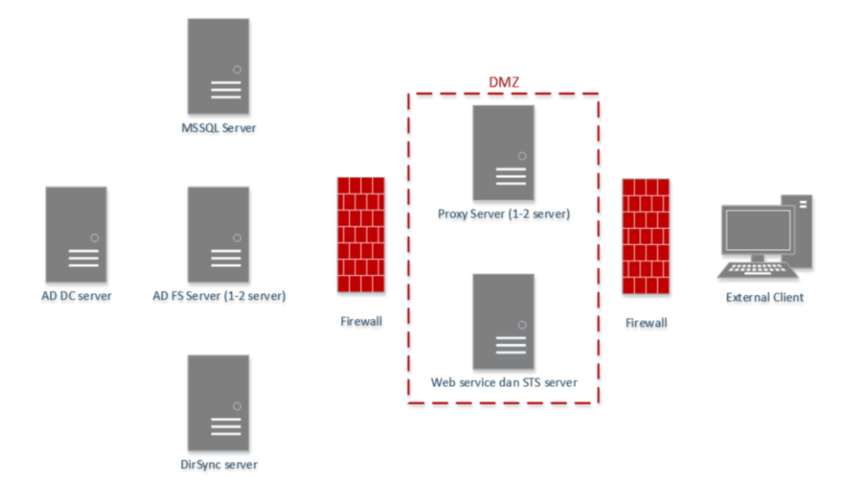
\includegraphics[width=12cm]{contents/chapter-2/gambar-buatan-sendiri.png}
	\caption[Contoh gambar]{Contoh gambar \cite{lukito2016}}
	\label{Fig:gambar-buatan-sendiri}
\end{figure}



\textit{Game design document} adalah sebuah bagian penting dalam pembuatan game baik itu elemen-elemen penyusunnya maupun proses pengembangannya. Game design yang telah dibuat, dijabarkan satu persatu mengenai tahapan dalam pembuatan game dan hasilnya disatukan dalam bentuk dokumentasi \textit{game design document} yang digunakan oleh \textit{developer} sebagai buku petunjuk bagaimana membuat \textit{game} \cite{lukito2016}.

Dalam buku \textit{Game Design Essentials} disebutkan \textit{game design document} merupakan metode yang menghubungkan elemen-elemen penyusun \textit{game}, baik itu \textit{art, sound, program, 
gameplay} sehingga semuanya terdokumentasi menjadi satu dan menjadi acuan bagi para \textit{developer} dalam membuat \textit{game} \cite{wibirama2013dual}. 

\subsection{Dasar Teori Lainnya}

\section{Analisis Perbandingan Metode}

Di dalam tinjauan pustaka hasil akhirnya adalah analisis secara kualitatif atau pun secara kuantitatif kelebihan dan kekurangan metode jika dikaitkan dengan masalah, batasan-batasan masalah dan solusi yang dinginkan. Analisis kuantitatif tidak wajib teapi mempunyai nilai tambah di dalam tugas akhir saudara. Bagian ini menjelaskan kenapa metode tersebut dipilih dan uraikan dengan lebih jelas metode pelaksanaan tugas akhir yang ingin Anda lakukan. 

\section{Pertanyaan Tugas Akhir (Jika Perlu)}

Pertanyaan tugas akhir bersifat opsional dan dapat ditambahkan untuk menekankan hal-hal yang hendak diketahui dari tugas akhir berdasar pada tujuan tugas akhir. Pertanyaan tugas akhir dikenal dengan RQ (\textit{Research Question}) dan harus memiliki keterkaitan dengan RO (\textit{Research Objective}). Satu RO dapat memiliki satu atau lebih dari satu RQ. 

